%----------------------------------------------------------------------------------------
% Corporate Design 2016 Presentation
%----------------------------------------------------------------------------------------
% Last update 22.11.2017
%
% Changelog:
%   22.11.2017: changed style of numbered slides
%   21.11.2017: added \toogleFooter to hide/show footer on teh following slides
%   30.06.2017: added \enum{#number} to link to an enuemrate item
%   20.04.2017: added numbered option too show slide number at bottom-right, also an example for usage in individual footers, i.e. with \setFooter
%   30.11.2016: improved documentation of titlepage picture and some minor changes
%   28.11.2016: fix for [t] alignment to \frame
%   23.11.2016: FKR release version
%   21.11.2016: improvements for adaptability to institute-level
%   18.11.2016: initial version
%
% For questions or bug reports
% mailto: mirco.altenbernd@ians.uni-stuttgart.de
%
%----------------------------------------------------------------------------------------
% Obligatory settings and includes
%------------------------------------------------------------------------------
\pdfminorversion=4
\documentclass[11pt,aspectratio=1610]{beamer}
\usepackage{multicol}
\usepackage{mathtools} 
\usepackage{mathrsfs} % used for mathscr
\newcommand{\FF}{\mathcal{F}}
\newcommand{\HH}{\mathscr H}
\newcommand{\LL}{\mathscr L}
\newcommand{\ii}{i}


\usepackage{amsmath,amssymb,amsthm}
\usepackage{pstricks,pst-node,pst-coil,pst-plot,pstricks-add}
\usepackage{geometry,epsfig}
\usepackage{bbm}
\usepackage{bm} %für \boldsymbol
\usepackage{cite}
\usepackage{xcolor} % Für Farbe
\usepackage{empheq} % Für Boxen
\usepackage{verbatim}
\usepackage{animate}


\newcommand{\C}{\mathbb{C}} % komplexe
\newcommand{\K}{\mathbb{K}} % komplexe
\newcommand{\R}{\mathbb{R}} % reelle
\newcommand{\Q}{\mathbb{Q}} % rationale
\newcommand{\Z}{\mathbb{Z}} % ganze
\newcommand{\N}{\mathbb{N}} % natuerliche
\DeclareMathOperator*{\esssup}{ess\,sup}
\newcommand{\B}[1]{ \textbf{#1}}


%\newcommand{\begin{proof}}{\textit{Proof. }}	%für Beweise	
%\newcommand{\end{proof}inalign}{\tag*{$\blacksquare$}} %eproof in align Umgebung nach rechts
%\newcommand{\end{proof}}{\hfill $\blacksquare$}	

\DeclareRobustCommand{\rchi}{{\mathpalette\irchi\relax}}
\newcommand{\irchi}[2]{\raisebox{\depth}{$#1\chi$}} %richtiges Chi
\newcommand{\intd}{\int \hspace{-1.5mm} d} %\int dx richtig plaziert
\newcommand{\all}{\quad \text{for all} \: \,} %Abkürzung von für alle
\newcommand{\Ima}{\operatorname{Im}}
\newcommand{\Rea}{\operatorname{Re}}

\renewcommand{\baselinestretch}{1.1}
\renewcommand{\qedsymbol}{\rule{1.3mm}{2.6mm}}


%
%------------------------------------------------------------------------------
% Basic slide layout configuration
%
% Important: remove all auxiliary files before recompilation when switching
%            from english (the default) to german and vice versa
%------------------------------------------------------------------------------
% \usetheme{fbm2016}                  % english talk
%\usetheme[simtech]{fbm2016}         % english, with additional SimTech logo
%\usetheme[german]{fbm2016}          % german
%\usetheme[numbered]{fbm2016}        % add slide count to the bottom right, only if '\setFooter' is not used. Otherwise see example in '\setFooter' to obtain similar results
\usetheme[german,simtech]{fbm2016}  % german, with SimTech logo
%
% feel free to implement GRK 1838 etc., by cloning the SimTech option
%
%------------------------------------------------------------------------------
% additional packages, anything beamer-compatible is allowed
%------------------------------------------------------------------------------
\usepackage{amsmath}  % just an example
\usepackage{amssymb}  % just an example
\usepackage{amsthm}   % just an example
%
%------------------------------------------------------------------------------
% Personalisation of title page, and inividual footers on all subsequent slides
%------------------------------------------------------------------------------

\title{Project 2: Time dependent heat equation with a source}
\subtitle{\small{Scientific Computing}
}
\author{V.~Ku{\ss}maul, N.~Thorin}
\date{\, }
% subtext below "Uni-Stuttgart" logo on frontpage
\setLogoText{Department of Mathematics}
% background image for titlepage, with and without size
\setTitlePic{../images/animation_frame.png}
% \defTitlePic{\includegraphics[height=6cm]{titlepic.jpg}}
% complete removal of the image
% \defTitlePic{}


% Define an individual footer. If not set a default footer is used which depends on the used beamer options: simtech, german, numbered
% Up to three optional logos/URLs/names in all footers of subsequent slides,
% please only edit lines marked as %%%%.
 \setFooter{
 	\vspace*{1cm} % for alignment issues: otherwise the content does not recognize the footer
   \begin{tikzpicture}[remember picture,overlay]
     % horizontal line
     \ifnum\thepage>1\draw (0.5,1) node(a) {} (15.5,1) node(b) {}; \draw[CD01!40] (a.east) -- (b.west);\fi
      %left aligned footer-content
      \node[anchor=south west, align=left, yshift=0.01\paperwidth, xshift=0.036\paperwidth] at (current page.south west) {
       %\includegraphics[height=0.05\paperheight]{logo_iadm.jpg}
        %%%%\includegraphics[height=0.05\paperheight]{f8banner.pdf}
       %%%%\includegraphics[height=0.05\paperheight]{mathebanner.pdf}
      };
      %center aligned footer-content
      \node[anchor=south, align=center, yshift=0.01\paperwidth, xshift=0] at (current page.south) {
        %%%%\includegraphics[height=0.05\paperheight]{logo_simtech.pdf}
        %\includegraphics[height=0.05\paperheight]{mathebanner.pdf}
        %%%%\includegraphics[height=0.05\paperheight]{logo_institute.pdf}
      };
      %alternative center aligned footer-content, yshift may be modified for alignment
      \node[anchor=south, align=center, yshift=0.025\paperwidth, xshift=0] at (current page.south) {
        %%%% {\bfseries\large www.sfbtrr75.de}\\
        %%%% {\bfseries\large www.simtech.uni-stuttgart.de}
      };
      %right aligned footer-content, not on title page
      \node[anchor=south east, align=right, yshift=0.01\paperwidth, xshift=-0.036\paperwidth] at (current page.south east) {
        %uni logo in footer only after title page
        \ifnum\thepage>1\includegraphics[height=0.06\paperheight]{logo_uni_english.pdf}\fi
      };
      %right aligned frame number on slides after title slide
      %%%% \ifnum\thepage>1\node[anchor=center, minimum size=2.cm] at (16.1,-0.3) {};
      %%%% \node[anchor=center] at (15.7,1) {\parbox[t][][t]{3cm}{\hspace*{-0cm}\centering\color{CD01}\scriptsize \insertframenumber}};\fi
    \end{tikzpicture}
 }

%------------------------------------------------------------------------------
%   Actual content
%------------------------------------------------------------------------------

\begin{document}

%%%%%%%%%%%%%%%%%%%%%%%%%%%%%%%%%%%%%%%%%%%%%%%%%%%%%%%%%%%%%%%%
%			titlepage
%%%%%%%%%%%%%%%%%%%%%%%%%%%%%%%%%%%%%%%%%%%%%%%%%%%%%%%%%%%%%%%%

\begin{frame}
	\titlepage
\end{frame}



\begin{frame}{Introduction} 
	We solve the \textbf{time dependent heat equation}
	\begin{align*}
	\begin{cases}
		\partial_t u - \Delta u = f,& \quad \text{in} \: \, \hspace{2mm} (0,1)^2,\\ 
		\hspace{13mm} u = g,& \quad \text{on} \: \, \partial (0,1)^2. 
	\end{cases}
	\end{align*}
	with a source $f$ and boundary condition $g$. 
	
\end{frame}

\begin{frame}{Discretization}
We use finite differences for the Laplacian
	\begin{align*}
		(\Delta u)(x) \approx  \big( u(x_1 - \delta x, x_2)& + u(x_1 + \delta x, x_2) + \\ 
			&u(x_1, x_2 - \delta x) + u(x_1, x_2 + \delta x) - 4 u(x_1, x_2) \big) / \delta x^2
	\end{align*}
and the time derivative 
	\begin{align*}  
		\frac{u(x, t + \delta t) - u(x, t)}{\delta t} - (\Delta u)(x, t + \delta t) \approx f(x, t + \delta t) \\ 
		\iff u(x, t + \delta t) - \delta t (\Delta u)(x, t + \delta t) \approx \delta t \,  f(x, t + \delta t) + u(x, t)
	\end{align*} 


\end{frame}





%---------------------------------------------------------Discretized grid --------------------------------------------
\begin{frame}

\begin{minipage}{0.5 \textwidth}
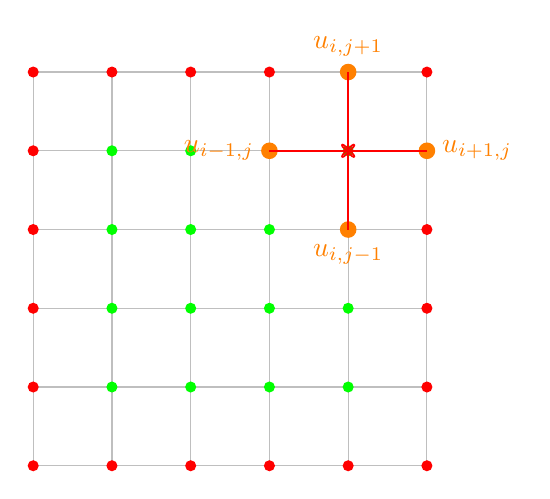
\begin{tikzpicture}

% Number of grid divisions
\def\n{5}

% Draw grid
\foreach \i in {0,...,\n} {
    \draw[gray!50] (\i,0) -- (\i,\n);
    \draw[gray!50] (0,\i) -- (\n,\i);
}

% Plot points and color them
\foreach \i in {0,...,\n} {
    \foreach \j in {0,...,\n} {
        % Check if boundary point
        \ifnum\i=0
            \fill[red] (\i,\j) circle (2pt);
        \else\ifnum\i=\n
            \fill[red] (\i,\j) circle (2pt);
        \else\ifnum\j=0
            \fill[red] (\i,\j) circle (2pt);
        \else\ifnum\j=\n
            \fill[red] (\i,\j) circle (2pt);
        \else
            \fill[green] (\i,\j) circle (2pt);
        \fi\fi\fi\fi
    }
}

% Central point (interior)
\def\cx{4}
\def\cy{4}

% Highlight center point
%\fill[blue] (\cx,\cy) circle (3pt) node[below left=2pt] {$u_{i,j}$};

% Highlight stencil neighbors (4-neighbor Laplacian)
\fill[orange] (\cx+1,\cy) circle (3pt) node[right=2pt] {$u_{i+1,j}$};
\fill[orange] (\cx-1,\cy) circle (3pt) node[left=2pt] {$u_{i-1,j}$};
\fill[orange] (\cx,\cy+1) circle (3pt) node[above=2pt] {$u_{i,j+1}$};
\fill[orange] (\cx,\cy-1) circle (3pt) node[below=2pt] {$u_{i,j-1}$};

% Optional: arrows to center
\foreach \dx/\dy in {1/0, -1/0, 0/1, 0/-1} {
    \draw[->, thick, red] ({\cx+\dx},{\cy+\dy}) -- (\cx,\cy);
}

% Optional: axes or labels
%\draw[->] (0,0) -- (\n+1,0) node[right] {$x$};
%\draw[->] (0,0) -- (0,\n+1) node[above] {$y$};

\end{tikzpicture}
\end{minipage}
\hfill
\begin{minipage}[c]{0.45 \textwidth}
Let $u_{i j}^{(\ell)} = u(x_{i j}, t_\ell)$, $0 \leq i, j < N$. Then
\begin{align*}  
	u_{i j}^{(\ell + 1)} - \frac{\delta t}{\delta x^2} (L u)_{i j}^{(\ell + 1)} = \delta t \, f_{i j}^{(\ell + 1)} + u_{i j}^{(\ell)} 
\end{align*} 
where $$(L u)_{i j} = u_{i - 1, j} + u_{i + 1, j} + u_{i, j - 1} + u_{i, j + 1} - 4 u_{i j}$$
and $u_{i j}^{(\ell)} = g_{i j}^{(\ell)}$ in boundary points. 

\vspace{10mm}
Transfer to 1D by $n = iN + j$.
\end{minipage}
\end{frame}

\begin{frame}{Discretization (summary)}
    Set
    \begin{equation*}
        A = I - \frac{\delta t}{\delta x^2} L.
    \end{equation*}

    Want to solve
    \begin{equation*}
       Au^{(\ell+1)} = u^{(\ell)} + \delta t\, f^{(\ell+1)}
    \end{equation*}

   \textbf{Note:} $A$ is spd! $\rightsquigarrow$ Use CG-method
\end{frame}





\begin{frame}[fragile]{Implementation details}
\footnotesize
\begin{verbatim}
def sparse_laplacian(self) -> csr_matrix:
    def in_bounds(i, j): 
        return (0 <= i < self.N) and (0 <= j < self.N)
    
    L = lil_matrix((self.N**2, self.N**2)) 
    boundary_points = defaultdict(list) 
    directions = [(-1, 0), (1, 0), (0, -1), (0, 1)]
    for i in range(self.N):
        for j in range(self.N):
            L[self.n(i, j), self.n(i, j)] = -4 
            for dx, dy in directions:
                i_, j_ = i + dx, j + dy
                if in_bounds(i_, j_):
                    L[self.n(i, j), self.n(i_, j_)] = 1
                else:
                    boundary_points[self.n(i, j)].append(((i_+1)*self.dx, (j_+1)*self.dx)) 
    self.boundary_points = boundary_points
    return (1/self.dx)**2 * csr_matrix(L) 
\end{verbatim}
\end{frame}

\begin{frame}[fragile]{CG Method}
\footnotesize
\begin{verbatim}
    def unpreconditioned_solve(self, b: np.ndarray, initial_guess: np.ndarray):
    	x = initial_guess
        r = p = b - self.A@x 
        alpha = np.dot(r, r) 

        for _ in range(self.max_iterations):
            v = self.A@p 
            _lambda = alpha / np.dot(v, p)
            x = x + _lambda * p
            r = r - _lambda * v
            alpha_new = np.dot(r, r)
            p = r + (alpha_new / alpha) * p
            alpha = alpha_new

            if alpha < self.tol**2:
                return x
            
        return None
\end{verbatim}
\end{frame}

\begin{frame}
      \animategraphics[loop,controls,autoplay,width=0.7\linewidth]{16.7}{../animation/animation-}{0}{149}
\end{frame}


\begin{frame}{Preconditioning}
\begin{itemize}
    \item $A$ is spd, we are doing CG $\rightsquigarrow$ Incomplete Cholesky as preconditioner.
    \item We use IC(0) $\rightsquigarrow$ Sparsity pattern is conserved.
    \item $A = L^TL$ $\rightsquigarrow$ $A \approx \tilde{L}^T\tilde{L} = P$
    \item Improvements: Smaller conditioning number $\rightsquigarrow$ Fewer iterations needed
    \item Downsides: Solve two sparse triangular systems $\rightsquigarrow$ More computing time per iteration
\end{itemize}



\end{frame}



%%%%%%%%%%%%%%%%%%%%%%%%%%%%%%%%%%%%%%%%%RESULTS%%%%%%%%%%%%%%%%%%%%%%%%%%%%%%%%%%%%%%
\begin{frame}{Results (conditioning number)}
	\begin{figure}
		\includegraphics[width=0.8\textwidth]{../images/conditioning_test.png}
	\end{figure}

\end{frame} 




\begin{frame}{Results (iterations)}
\begin{figure}
	\includegraphics[width=0.8\textwidth]{../images/iterations_test.png}
\end{figure}
\end{frame}

\begin{frame}{Results (residual)}
\begin{figure}
	\includegraphics[width=0.8\textwidth]{../images/residual_test.png}
\end{figure}
\end{frame}

\begin{frame}{Results (time)}
\begin{figure}
	\includegraphics[width=0.8\textwidth]{../images/time_test.png}
\end{figure}
\end{frame}

\begin{frame}{Profiling}
\begin{figure}
    \includegraphics[width=\textwidth]{../images/line_profiler.png}
\end{figure}

\end{frame}




%%%%%%%%%%%%%%%%%%%%%%%%%%%%%%%%%%%%%%%%%%%%%%%%%%%%%%%%%%%%%%%%
%					References
%%%%%%%%%%%%%%%%%%%%%%%%%%%%%%%%%%%%%%%%%%%%%%%%%%%%%%%%%%%%%%%%

\begin{frame}{References}

%\bibliography{scicomp_references}
%\bibliographystyle{plain}

\begin{thebibliography}{1}

\bibitem{scicomp}
Dominik Göddeke.
\newblock Scientific computing.
\newblock Lecture Notes, June 2024.
\newblock Version: 25th June 2024.

\end{thebibliography}


\vspace{10mm} 

\textbf{ChatGPT} was used for implementation details regarding sparse matrices and visualizing our numerically computed solution. 


\end{frame}







%\begin{frame}{References}
%\bibliography{pointwise_refrences}
%\bibliographystyle{plain}
%\end{frame}





\end{document}












%----------------------------------------------------------------------------------------
%   Content (end)
%----------------------------------------------------------------------------------------
